\chapter{Simulator}\label{ch:simulator}
In this chapter we explain the core part of the code which is devoted to define the classes necessary to implement our discrete equations, the linear and the nonlinear solver and the storing of the solution. We will give a general overview of the main methods, the logic behind them and how all the classes are related.

We design our code to achieve a great flexibility since the final goal of the project is to obtain a framework for multi-physics simulations. For this reason we wrote a code strongly object-oriented with base classes very generic to permit a simple implementation of new basis, quadrature formulas, discrete equations, etc. . To achieve this results we used templates since they are statically bound and we tried to avoid virtual function, which are dynamically bound. Cmp. \cite{cpp_primer}.

In Fig.(\ref{fig:sem_diagram}) it is shown a simplified diagram of the main classes which will be explained in this chapter.

\begin{figure}
\centering
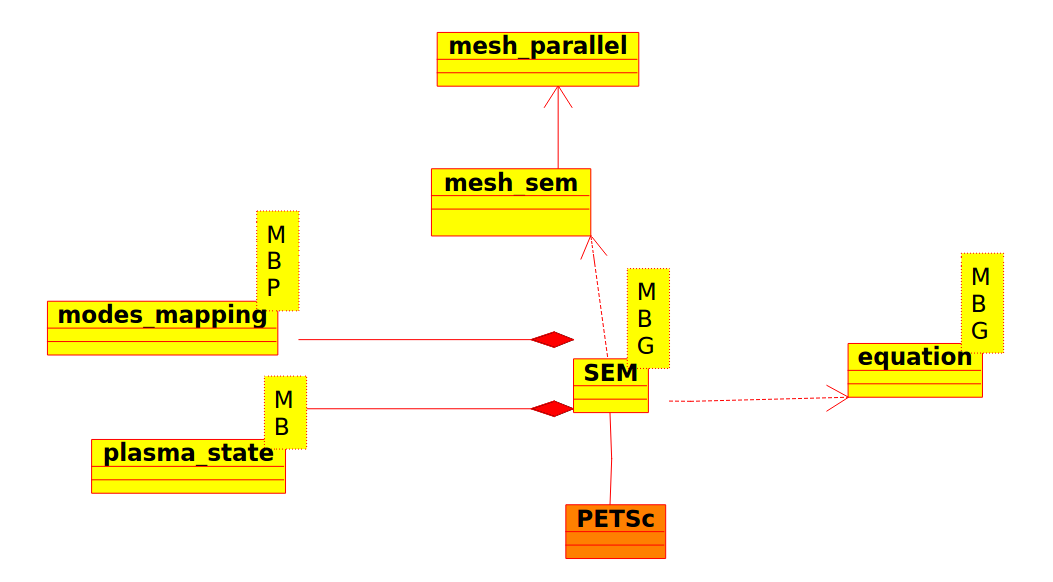
\includegraphics[scale=0.3]{images/sem_diagram.png}
\caption{Simulator: classes structure.}\label{fig:sem_diagram}
\end{figure}

\section{Mesh}\label{sec:mesh}
The mesh is defined in the class \verb|mesh_sem| which inherits from the class \verb|mesh_parallel|. The class \verb|mesh_parallel| already contains all the methods and all the informations needed by our method; the only additional information needed is the local degree of the basis. Therefore this derived class contains a vector where are stored all the elements degrees which are locally stored. Since we need also to know the degrees of each ghost we used the class \verb|ghost_communication| to keep updated these values. Moreover there are implemented some inline methods to extract the maximum degree, the local degree of an element and the degree of the edge which is the minimum degree of the two elements which share that edge.

\section{Polynomial basis}\label{sec:modal_basis}

We choose to adopt a modal basis which is built in a recursive way using the Legendre polynomials $\{L_k\}_0^p$ which are defined, over the logical domain $[-1,1]$, as
\begin{equation}
  \begin{cases}
    L_0(\hat{x})=1\\
    L_1(\hat{x})=\hat{x}\\
    (k+1)L_{k+1}(\hat{x})=(2k+1)\hat{x}L_k(\hat{x})-kL_{k-1}(\hat{x}),\quad k=1,\dots,p_m-1
  \end{cases}
\end{equation}
with derivatives
\begin{equation}
  (1-\hat{x}^2)L'_k(\hat{x})=kL_{k-1}(\hat{x})-k\hat{x} L_k(\hat{x}),\quad k\geq 1.
\end{equation}
These polynomials form a modal basis of $\mathbb{P}_p(-1,1)$, indeed it is hierarchic, which means that the expansion set of order $p$ is contained within the expansion set of order $p+1$. By definition they are orthogonal respect the Legendre inner product, $(u,v)_w=\int uvw$ with $w\equiv 1$ so it is the usual inner product in $L^2(-1,1)$.
\medskip

The Legendre polynomials are implemented in the class \verb|legendre| which contains four variables, stored as \verb|vector<vector<double> >|, to store the coefficients of the Legendre polynomials and their derivatives both in ascending and descending orders. The $i^{th}$-row store the coefficients of polynomials $L_i$. We store the coefficients in both order because sometimes it is necessary to pass this array of coefficients to some C library functions which operates with ascending or descending order array.

The main method are the ones which returns the vector of coefficients: \verb|c(j)|, \verb|c_der(j)|, \verb|c_reverse(j)| and \verb|c_der_reverse(j)| where \verb|j| is the number of the polynomials. If \verb|j| is bigger than the maximum value stored, the new coefficients are evaluated and added to the vectors, before returning the reference.
\medskip

Unfortunately the Legendre modal basis cannot be extended, without great difficulties, to an elemental decomposition which is globally $C^0$ therefore we adopt a new defined using the Legendre polynomials. We defined our basis with the following recursive formula
\begin{equation}\label{eq:modal_basis_1D}
  \begin{cases}
    \phi_0(\hat{x})=\frac{1-\hat{x}}{2}\\
    \phi_1(\hat{x})=\frac{1+\hat{x}}{2}\\
    \phi_k(\hat{x})=\frac{1}{\sqrt{2(2k-1)}}(L_{k-2}(\hat{x})-L_k(\hat{x})), & k=2,\dots,p
  \end{cases}
\end{equation}
which defines a modal hierarchic boundary-adapted basis.

\begin{figure}
\centering
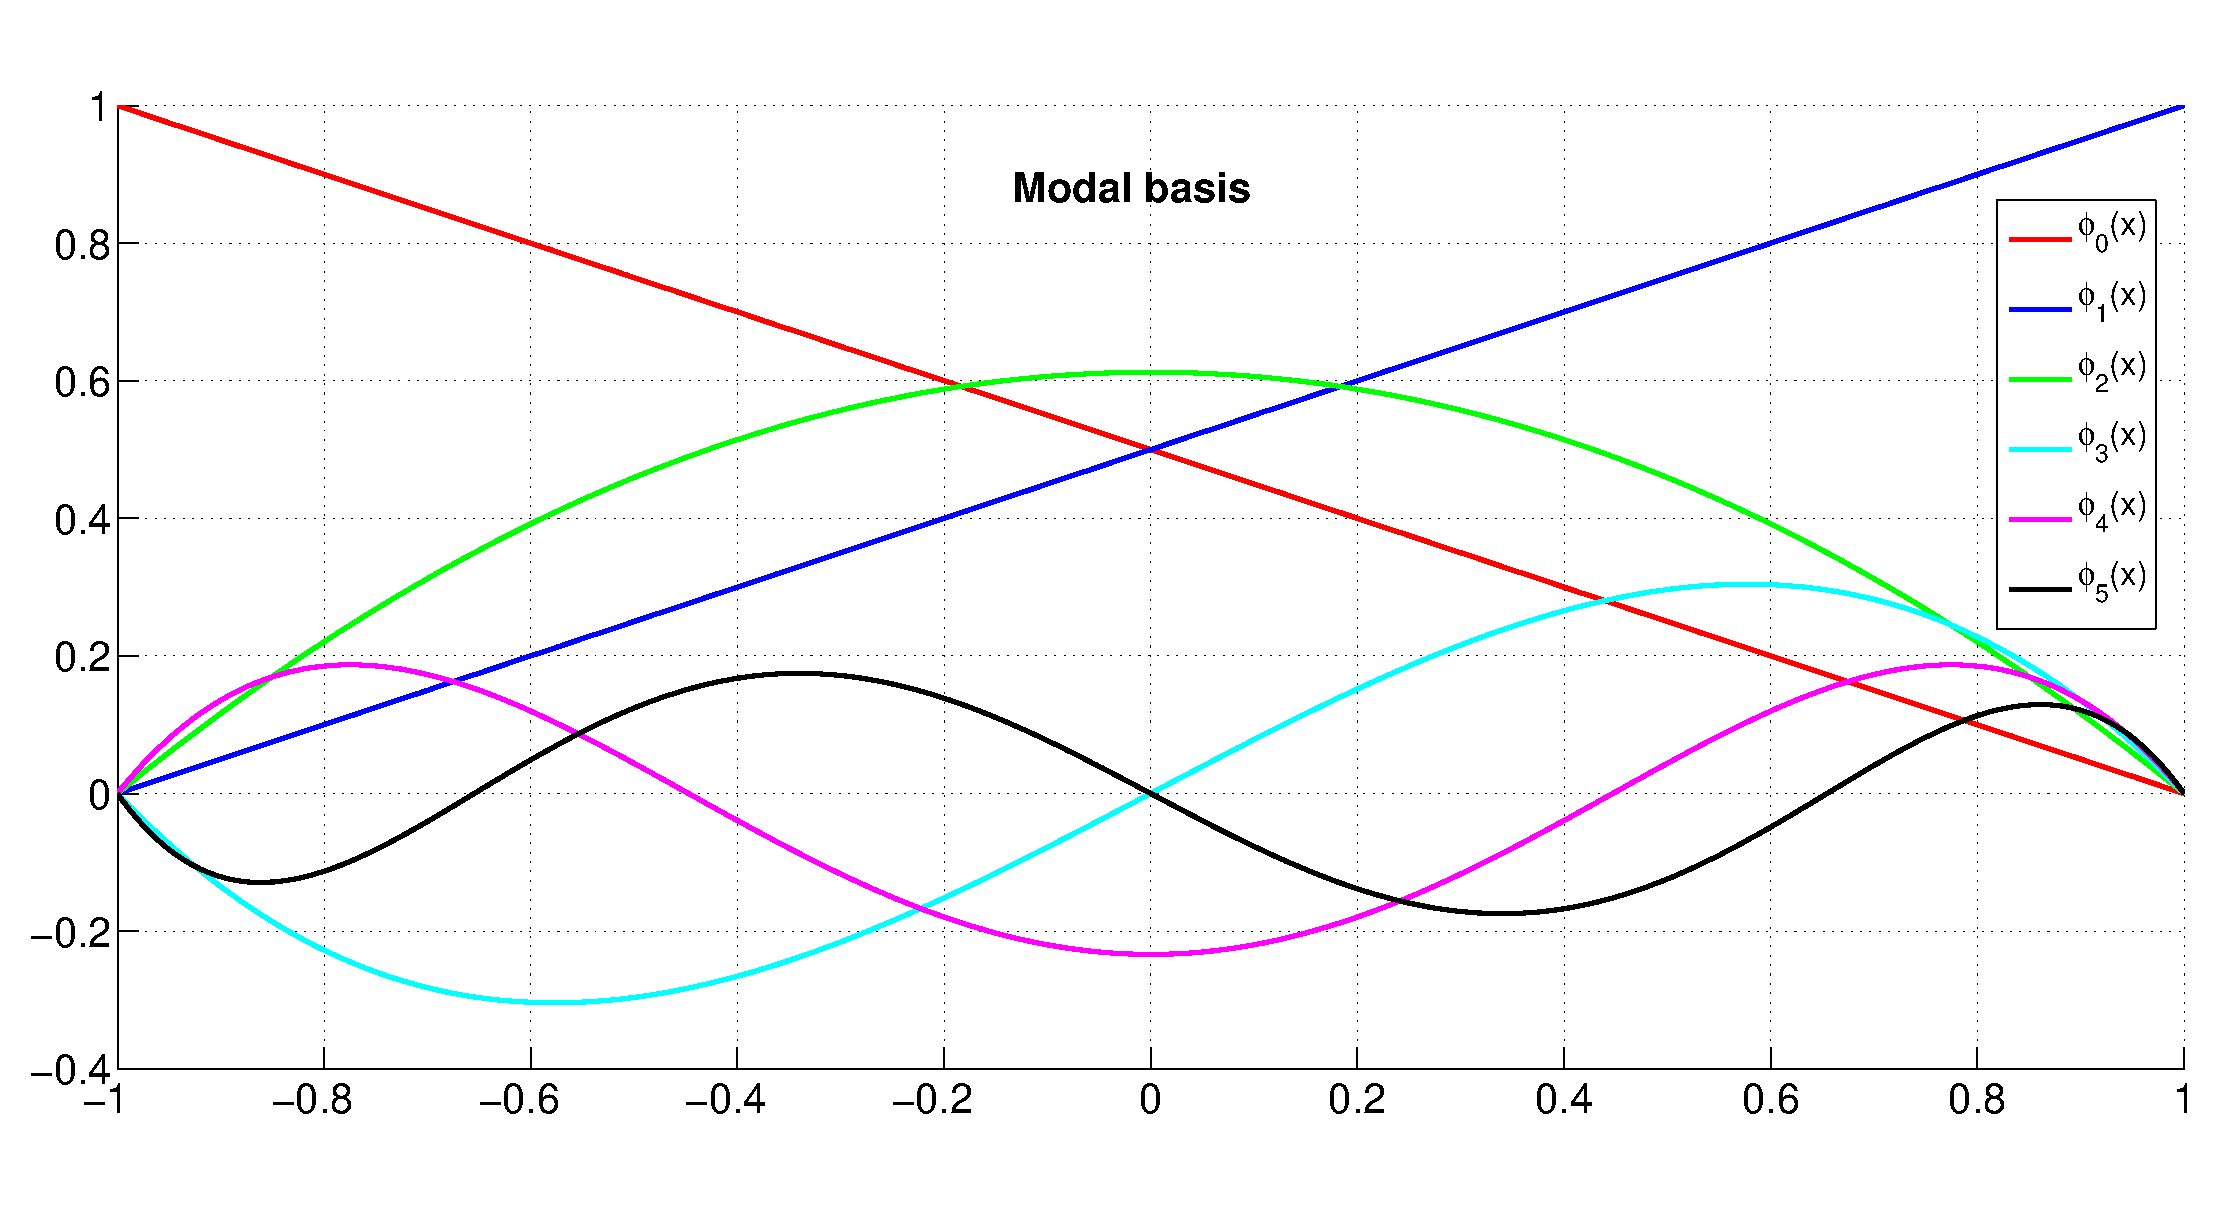
\includegraphics[scale=0.3]{images/1D_basis.eps}
\caption{Modal basis $\phi_i(\hat{x})$, with $i\in\{0,\dots,5\}$, defined on the interval [-1,1].}\label{fig:1D_basis}
\end{figure}

The first six modes are plotted in Fig.(\ref{fig:1D_basis}). A hierarchic basis is convenient, from a computational point of view, to increase locally the degree of polynomials which is necessary when one needs to perform a p-refinement. Indeed, for a hierarchic basis, it holds that the basis of $\mathbb{P}_p$ is a subset of $\mathbb{P}_{p+1}$ therefore
\begin{equation}
  \{\phi_i\}_0^p\subset\{\phi_i\}_0^{p+1}=\{\phi_i\}_0^p\cup\{\phi_p+1\}.
\end{equation}

A basis of $\mathbb{P}_p(-1,1)$ is defined boundary-adapted if contains two modes, called \textit{vertex functions}, that are nonzero at precisely one endpoint of the interval (red and blue functions plotted in Fig.(\ref{fig:1D_basis})), and $p-1$ modes, called \textit{bubble functions}, that vanish at both endpoints (green, light blue, magenta and black functions plotted in Fig.(\ref{fig:1D_basis})). The drawback of the new basis is that it is not orthogonal.
\medskip

It is possible to demonstrate that the derivatives of our basis can be evaluated using the following iterative formula
\begin{equation}
  \begin{cases}
    \phi'_0(\hat{x})=-\frac{1}{2}\\
    \phi'_1(\hat{x})=\frac{1}{2}\\
    \phi'_k(\hat{x})=-\sqrt{\frac{2k-1}{2}}L_{k-1}(\hat{x}), & k=2,\dots,p.
  \end{cases}
\end{equation}
\medskip

We implement a base class, called \verb|basis_function|, which is a pure abstract class for basis management. It contains two matrices, type \verb|vector<vector<double> >|, to store the coefficients of the basis and the coefficients of its derivatives in descending order. It has two methods to evaluate the value of the basis and the value of its derivative in a certain point of the logical domain, respectively \verb|eval(x,j)| and \verb|eval_der(x,j)|. It has a pure abstract method, \verb|set_basis_order(j)|, which must be overload; it fills the vector of coefficients of the basis. Before using the methods to evaluate the basis or its derivative in a certain points it is necessary to call once the method \verb| set_order(j)|. This method call the overloaded method \verb|set_basis_order| to fill the vector with the coefficients of the basis and than it computes and stores the coefficients of the derivatives of the basis in another vector.
\medskip

Our basis is implemented in the class \verb|leg_modal_basis| which inherits from the pure abstract class \verb|basis_function|. It simply has a variable of type \verb|legendre| and the method \verb|set_basis_order| which is the implementation of the recursive formula to evaluate the basis Eq.(\ref{eq:modal_basis_1D}).
\medskip

From the one-dimensional basis we can build the two-dimensional basis. Let's start defining on the logical element, the square $\hat{\Omega}=[-1,1]\times[-1,1]$, the space of polynomials of degree $\leq N$ in each coordinate $\mathbb{Q}_N$, for $N\geq 1$. We cannot have different maximum degrees on the two space variables because it is integral to definition of $\mathbb{Q}_N$. More precisely $\mathbb{Q}_N$ is defined as
\begin{equation}
  \mathbb{Q}_N(\hat{\Omega})=\mathrm{span}\{\hat{x}^i \hat{y}^j, \: 0\leq i,j\leq N,(\hat{x},\hat{y})\in \hat{\Omega}\}
\end{equation}
and its dimension is $(N+1)^2$.

For that space $\mathbb{Q}_N(\hat{\Omega})$ we choose to adopt a boundary-adapted modal basis. The basis is simply constructed using the tensor product of one-dimensional basis; the resulting functions are defined on Cartesian products of intervals. Precisely, given two families$\{\phi_i(\hat{x})\}_0^p$ and $\{\phi_j(\hat{y})\}_0^p$ with $0\leq i,j\leq N$, the family $\{\phi_{ij}(\hat{x},\hat{y})\}_0^p$ is defined as
\begin{equation}
  \phi_{ij}(\hat{x},\hat{y})=\phi_i(\hat{x})\phi_j(\hat{y}),\qquad i,j=0,\dots,N
\end{equation}
In Fig.(\ref{fig:2D_basis}) is shown the basis in the special case of $p=2$.

\begin{figure}
\centering
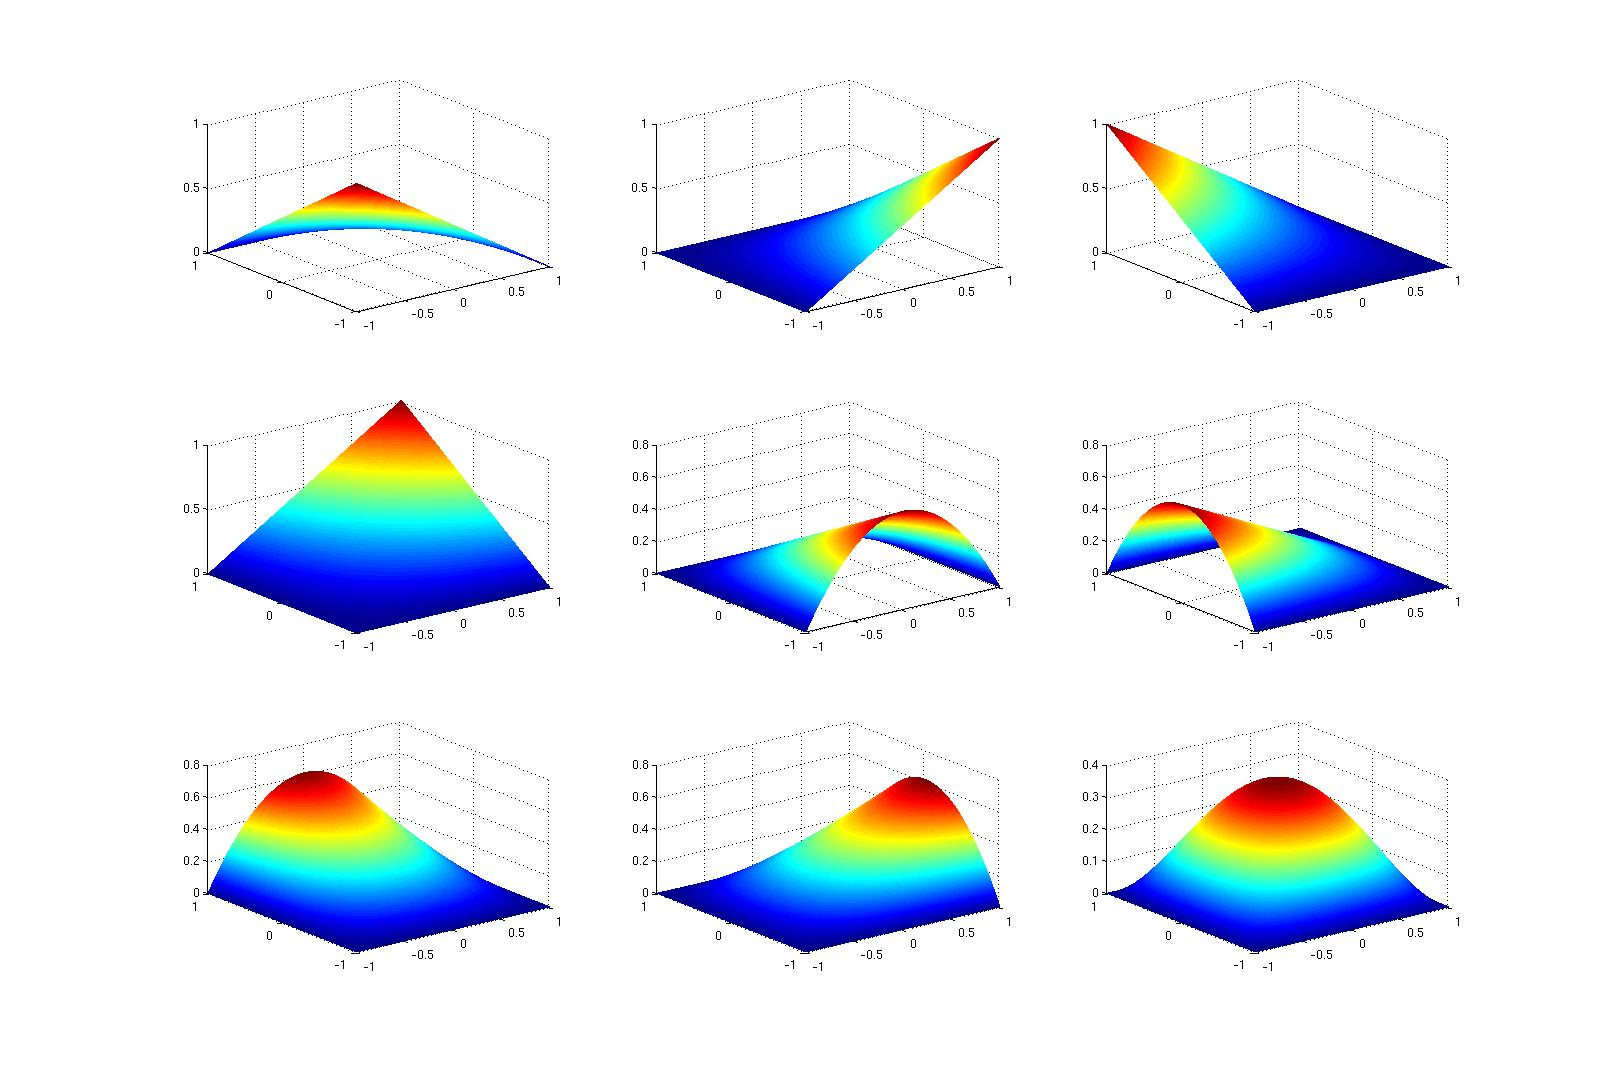
\includegraphics[scale=0.25]{images/2D_basis.jpg}
\caption{Modal basis $\phi_i(\hat{x})\phi_j(\hat{y})$, with $i,j\in\{0,\dots,2\}$, defined on the logical domain $[-1,1]\times[-1,1]$.}\label{fig:2D_basis}
\end{figure}

The usage of a modal basis corresponds to projection operator of $\psi$ over the space $\mathbb{Q}_N$.
\medskip

Any boundary-adapted basis is formed by three different type of modes:
\begin{itemize}
  \item $(N-1)^2$ \textit{bubble functions}, $(i\geq 2)\wedge(j\geq 2)$, which vanish on the boundary $\partial\hat{\Omega}$;
  \item 4 \textit{vertex functions}, $(i\leq 1)\wedge(j\leq 1)$, which do not vanish at precisely one vertex;
  \item $4(N-1)$ \textit{edge functions}, $\big((i\leq 1)\wedge(j\geq 2)\big)\vee\big((i\geq 2)\wedge(j\leq 1)\big)$ which do not vanish at precisely one edge.
\end{itemize}

In Fig.(\ref{fig:2D_basis}), starting from the top on the left and going to the bottom of the right, we have the 4 vertex functions, then 4 edge functions and last the unique bubble function which form the modal basis in the special case of $p=2$. Instead, Fig.(\ref{fig:modes_diagram}) is a diagram which shows where the modes are different from zero. Therefore we can see each vertex function to which vertex of the logical domain refers, each edge function to which edge of the logical domain refers and finally the bubble functions in the center of the domain since they vanish on the border.

\begin{figure}
\centering
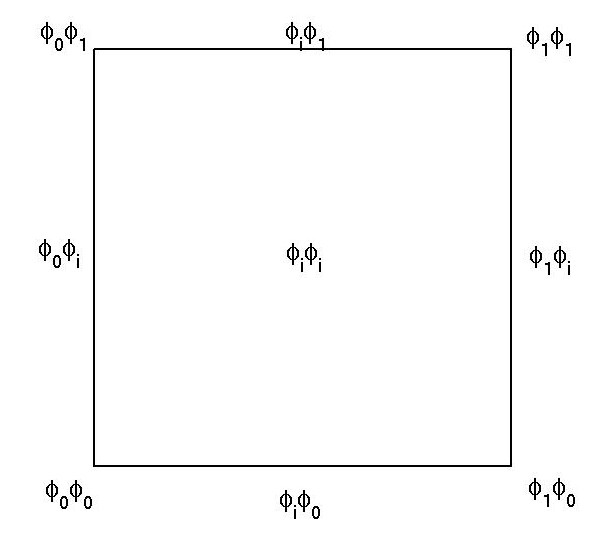
\includegraphics[scale=0.25]{images/modes_diagram.jpg}
\caption{Diagram of the modes, $i\geq 2$.}\label{fig:modes_diagram}
\end{figure}

The quadrilateral basis is therefore defined as:
\begin{description}
 \item[vertex]
   \begin{equation}
      \begin{cases}
	\phi_0(\hat{x})\phi_1(\hat{y})=\frac{1-\hat{x}}{2}\frac{1+\hat{y}}{2}\\
	\phi_1(\hat{x})\phi_1(\hat{y})=\frac{1+\hat{x}}{2}\frac{1+\hat{y}}{2}\\
	\phi_1(\hat{x})\phi_0(\hat{y})=\frac{1+\hat{x}}{2}\frac{1-\hat{y}}{2}\\
	\phi_0(\hat{x})\phi_0(\hat{y})=\frac{1-\hat{x}}{2}\frac{1-\hat{y}}{2}
      \end{cases}
   \end{equation}
  \item[edge]
    \begin{equation}
	\begin{cases}
	  \phi_i(\hat{x})\phi_1(\hat{y})=\frac{\sqrt{2(2i-1)}}{i}\frac{1-\hat{x}}{2}\frac{1+\hat{x}}{2}P^{1,1}_{i-2}(\hat{x})\frac{1+\hat{y}}{2}\\
	  \phi_1(\hat{x})\phi_i(\hat{y})=\frac{1+\hat{x}}{2}\frac{\sqrt{2(2j-1)}}{j}\frac{1-\hat{y}}{2}\frac{1+\hat{y}}{2}P^{1,1}_{j-2}(\hat{y})\\
	  \phi_i(\hat{x})\phi_0(\hat{y})=\frac{\sqrt{2(2i-1)}}{i}\frac{1-\hat{x}}{2}\frac{1+\hat{x}}{2}P^{1,1}_{i-2}(\hat{x})\frac{1-\hat{y}}{2}\\
	  \phi_0(\hat{x})\phi_i(\hat{y})=\frac{1-\hat{x}}{2}\frac{\sqrt{2(2j-1)}}{j}\frac{1-\hat{y}}{2}\frac{1+\hat{y}}{2}P^{1,1}_{j-2}(\hat{y})
	\end{cases}
    \end{equation}
  \item[interior]
    \begin{equation}
      \phi_i(\hat{x})\phi_j(\hat{y})=\frac{\sqrt{2(2i-1)}}{i}\frac{1-\hat{x}}{2}\frac{1+\hat{x}}{2}P^{1,1}_{i-2}(\hat{x})\frac{\sqrt{2(2j-1)}}{j}\frac{1-\hat{y}}{2}\frac{1+\hat{y}}{2}P^{1,1}_{j-2}(\hat{y})
    \end{equation}
\end{description}
where $P^{\alpha,\beta}_k(\hat{x})$ is the $k$-th order Jacobi polynomial and $i,j\geq 2$.
\medskip

We want to point out that, to have a lighter notation, we dropped the $\:\hat{}\:$ over the function $\phi$ since it is obvious that they are defined over the logical domain. Since it is possible to find an univocal mapping $(i,j)\longrightarrow i'$ which maps the numbering of the modes, in Ch.(\ref{chapter:sem}) we didn't explicitly write the basis like a tensor product but simply as $\hat{\phi}_{i'}(\mathbf{\hat{x}})$.

\section{Gaussian integration}\label{sec:gaussian_integration}
In order to evaluate the inner products of the discrete variational formulation, we choose the Gauss-Legendre-Lobatto (GLL) formula which is a Gaussian quadrature formula which has two nodes at the boundary on the interval. The $N+1$ GLL nodes $\{\hat{x}_n\}_0^N$ for the interval $[-1,1]$ are the endpoints of interval, to ensure the continuity between elements, and the maxims and minims of the $N$-th degree Legendre polynomial therefore the roots of the first derivative of $L_N$ while the weights are defined as
\begin{equation}
  w_n=\frac{2}{N(N+1)}\frac{1}{L^2_N(\hat{x}_n)}.
\end{equation}
Its degree of precision is $2N-1$ which implies that the discrete inner product is equal to the classical inner product if the product of the two function belongs to $\mathbb{P}_{2N-1}$.
\medskip

The GLL nodes and weights are evaluated using the class \verb|gaussian_integration| which contains two matrices, type \verb|vector<vector<double> >|, where are stored the nodes and the weights and a variable of type \verb|legendre| which is used to evaluate the Legendre polynomials. The zeros of the $L'_N$ are evaluated numerically using the function \verb|gsl_poly_complex_solve| of the library \verb|GSL| which accept an array of coefficients and return the zeros of the polynomials. Moreover there are some inline methods which returns, given the order of the polynomial to integrate, the necessary number of nodes to obtain an exact integration.

The methods \verb|get_nodes(j)| and \verb|get_weights(j)| return the reference to the \verb|j|-th row.
\medskip

Like for the modal basis, the GLL nodes and weights for the logical domain $\hat{\Omega}=[-1,1]\times[-1 1]$ are obtained taking the tensor product of the one-dimensional nodes and weights.

\section{Definition of the equations}
In Fig.(\ref{fig:equation_diagram}) it is reported the diagram which shows the structure of the classes involved in the definition of the equations.

\begin{figure}
\centering
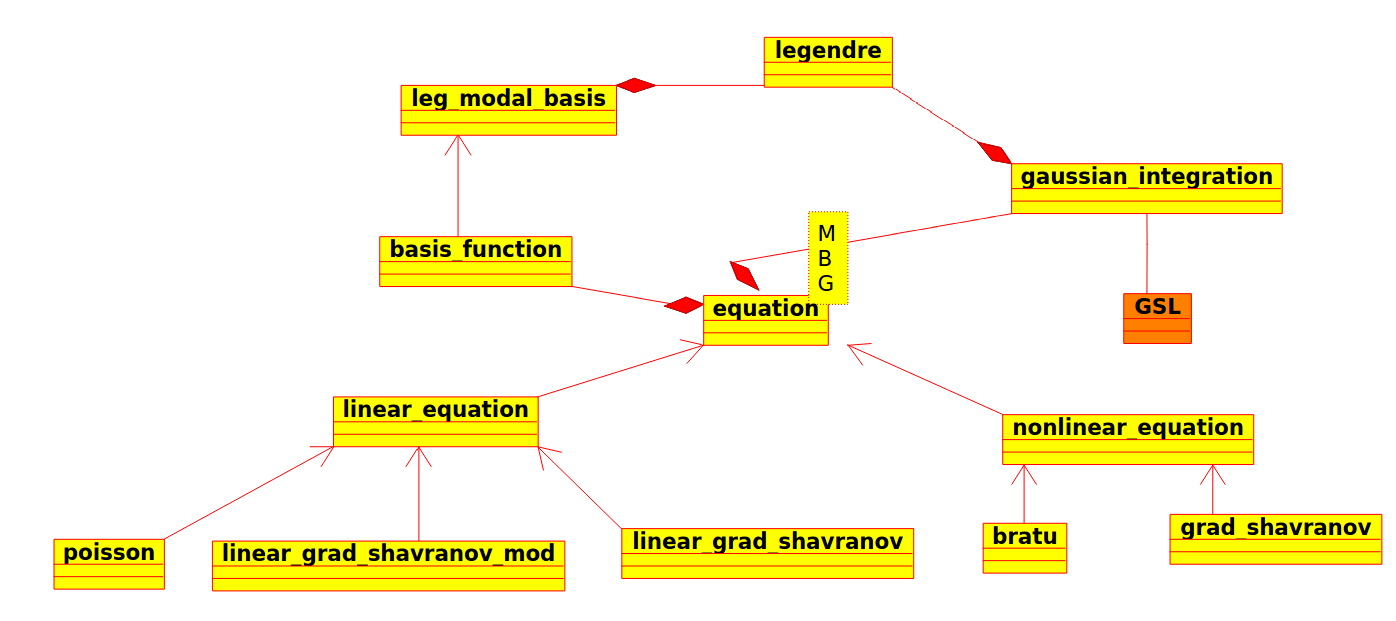
\includegraphics[scale=0.3]{images/equation_diagram.png}
\caption{Equation: classes structure.}\label{fig:equation_diagram}
\end{figure}

The base class is \verb|equation|; its constructor takes like arguments only a pointer to the mesh. It has two protected templated variables for the basis and for the numerical integration. When the constructor is called it extracts from the mesh the maximum degree of the basis needed. After that it constructs the basis variable according to that degree and it also constructs the numerical integration variable with the necessary number of points to obtain an exact polynomial integration up to that degree. Since the modes and their first derivatives will be evaluated in the same quadrature points a lot of time, these values are stored in a three-dimensional matrix where the first dimension is the mode number, the second is the number of quadrature points desired and the third the values of the mode in the nodes. The same matrix is evaluated for the first derivatives. These matrices are filled using the method \verb|compute_basis|.

Another method called automatically in the constructor is \verb|compute_dirichlet_coeff|, which, for each boundary lines, computes the coefficients of the projection of the Dirichlet condition over the basis. These projection coefficients are stored in a private variable of type \verb|vector<vector<double> >|.
\medskip

The class \verb|linear_equation| and \verb|nonlinear_equation| inherit from this base class. They are very similar since they implements the routines used to evaluate the contribution of the stiffness matrix and the RHS.

The class for the linear equations have three pure virtual methods \verb|eval_LHS|, \verb|eval_RHS| and \verb|eval_neumann| which must be overload in the derived classes. In these methods there must be written the parts of the discrete formulation inside the summations. This methods are used by \verb|LHS|, \verb|RHS| and \verb|neumann| which evaluate the Jacobian of the transformations and loop over the elements and the quadrature nodes. These are the methods used to evaluate the contribution inside the stiffness matrix and the right hand term of the final linear system.

Similarly, the class \verb|non_linearequation| has the methods \verb|LHS|, \verb|RHS| and \verb|neumann| but now they have a different meaning since the LHS for the non linear equation is the Jacobian of the Newton abstract methods while the RHS is the functional of the method multiplied by $-1$ . The method which must be overload are called \verb|eval_Jacobian|, \verb|eval_F0| and \verb|eval_neumann|.
\medskip

We have implemented several different equations deriving their classes from the previous two in accordance to the nature of the equation. In Sec.(\ref{sec:exemples}) we describe each equations which we have implemented.

\section{Global operation}\label{sec:global_assembling}
To construct a globally $C^0$ continuous expansion from elemental contributions, we must match the local boundary modes with a similar shape: vertex and edge modes. Therefore we need to assemble the global system from the local systems creating a map between the global system and the local systems. The definition of this mapping is central to the global assembly process. If two neighboring elements have different local degree  a functional incompatibility between adjacent elements is created because of the continuity constraint which states that we have to match up all boundary modes. The solution is zeroing the coefficients of hanging degrees of freedom.
\medskip

Moreover it is important to notice that two edges modes must be glued together with the right sign when the degree of the modes is odd since the relative reference frame can be different. This fact is well shown in Fig.(\ref{fig:basis_assembling}) where there are represented two different situations which can happen when ones tries to glue together two edge modes of order 3. In the first case the two references frame are oriented in such a way that the modes has the same shape therefore no further operation is needed. Instead in the second case the two modes are reversed therefore it is necessary to subtract the modes instead of add them. We choose to adopt the convention that the leading reference frame is the one of the element with lower global index and the mode of the other element is glued according this conventional reference frame.

\begin{figure}
\centering
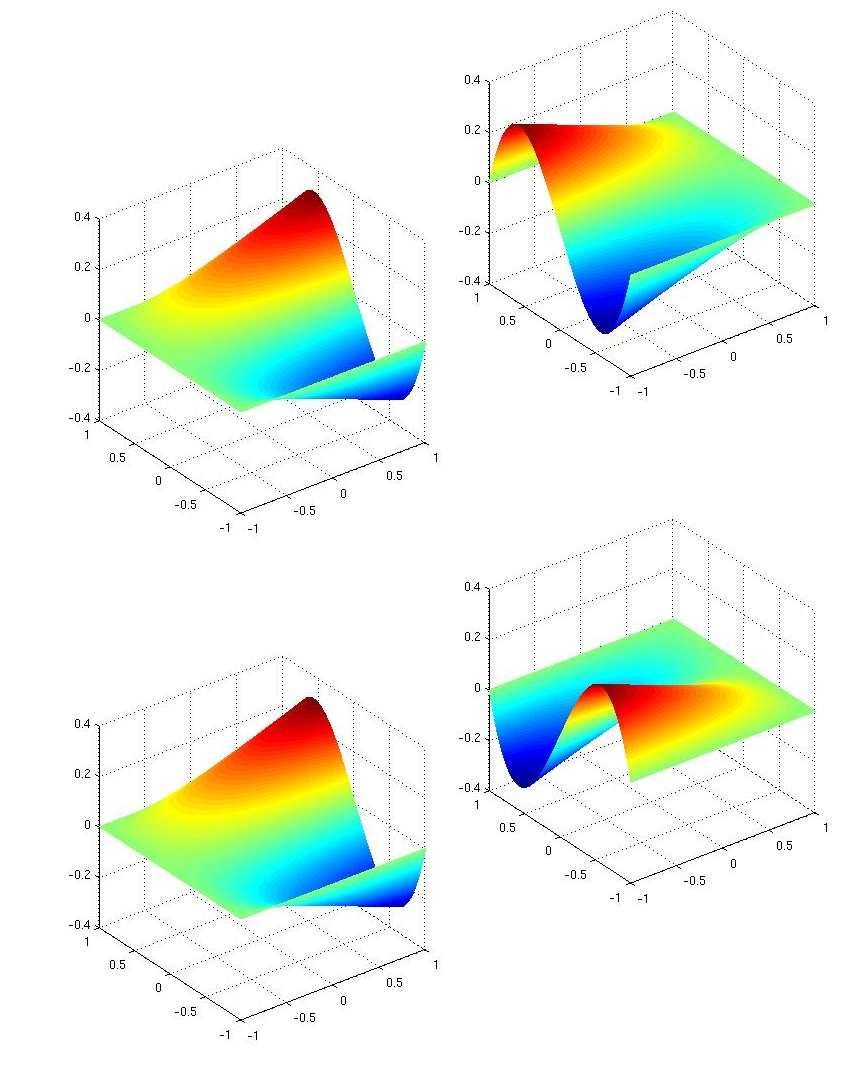
\includegraphics[scale=0.25]{images/basis_assembling_mod.jpg}
\caption{Global assembling for the edge mode $\phi_3(\hat{x})\phi_0(\hat{y})$ with two different local reference frames.}\label{fig:basis_assembling}
\end{figure}

The mapping which leads to a $C^0$ global basis is implemented in the class \verb|modes_mapping|. The constructor of the class calls the method \verb|create_mapping| which create the mapping. We number the modes following this order
\begin{itemize}
  \item vertex modes which are not degree of freedom;
  \item edge modes which are not degree of freedom;
  \item vertex modes which are degree of freedom;
  \item edge modes which are degree of freedom;
  \item bubble modes.
\end{itemize}
Therefore from the global number of the mode is straightforward to understand its type. This helps a lot during the stiffness assembling process.
\medskip

The map of the nodes is simply stored in a vector which has as many elements as the total number of the nodes; this vector is equal in each process. The map of the edge modes and bubble modes is stored in a matrix; each row represent one local element and has five entries. Each entry is the starting index of the modes corresponding to the first, second, third and fourth edge, with the convention adopted in Sec.(\ref{section:mono_cpu}). The fifth entry is the starting index of the bubble modes. The other global indices can be obtained from this matrix just adding the local numbering of the modes. For example if the mode $\phi_2\phi_0$, which is an edge mode, has global index $i$, the mode $\phi_5\phi_0$, which is an edge mode on the same edge, has global index $i+3$ since is the third mode of that edge.
\medskip

Other two important methods of the class are \verb|u(i,ii,e)|, which returns the coefficient of the solution referred to the modes $(\phi_i\phi_{ii})^e$, and \verb|u_sol(x,y,e)|, which returns $\hat{\psi}^e_{\delta}(\hat{x},\hat{y})$

\section{SEM simulator}
The part of the code devoted to the assembling of the linear system and the solution of it is implemented in the class \verb|SEM|. The constructor needs a pointer to the mesh, a pointer to the equation and a flag which can be \verb|STATIC_CONDENSATION_OFF|, default,  or \verb|STATIC_CONDENSATION_ON|. The constructor firstly creates the class \verb|mapping| and than create the necessary \verb|PETSc| variables calling the method \verb|create_petsc_variables|. The variables created depend on the type of the equation and on the flag:
\begin{itemize}
  \item linear equation without static condensation, created the matrix \verb|Abb| and the vectors \verb|Xb| and \verb|Fb|;
  \item linear equation with static condensation, created the matrices \verb|Abb|, \verb|Abi| and \verb|Abi| and the vectors \verb|Xb|, \verb|Xi|, \verb|Fb| and \verb|Fi|;
  \item nonlinear equation without static condensation, like the linear case without static condensation but in addition created the vector\verb|Xb_sol|;
  \item nonlinear equation with static condensation, like the linear with static condensation case but in addition created the vectors \verb|Xb_sol|, \verb|Xi_sol|.
\end{itemize}
All the matrices are of type \verb|MATMPIAIJ|, parallel sparse matrix, and all the vectors are of type \verb|VECMPI|, parallel vector.
\medskip

After the creation of the variables, the method \verb|create_scatter()|, using the \verb|PETSc| function \verb| VecScatterCreateToAll|, creates a scatter from the solution vector, which is parallel, to a sequential vector. This is necessary to retrieve the coefficients of the solution which are not locally stored. The solution vector for the linear case is \verb|Xb| (also \verb|Xi| with static condensation) while for the nonlinear case is \verb|Xb_sol| (also \verb|Xi_sol| with static condensation).
\medskip

The following step is the assembling of the matrix/matrices and of the vectors; to do this it is necessary the map created in the class \verb|modes_mapping| to put each contribution, evaluated through the class derived from \verb|equation|, in the right place. It is important to point out that the geometrically partition is not respected by the assembling process therefore a little more communication than necessary is carried out during this phase. Create a mapping which respects the geometric partition takes a lot more time than the one we created; for this reason we have chosen to do not respect the partition to speed up the code. The Dirichlet condition are imposed using the zeroing technique.
\medskip

Once that all the vectors and matrices are created, if the static condensation is off, the code simple solves the system using a \verb|PETSc| iterative linear solver, cmp. Sec.(\ref{sec:exemples}). If the static condensation is on it solves two systems. The idea behind static condensation technique is to rewrite the starting linear system
\begin{equation}
  A\mathbf{x}=\mathbf{F}.
\end{equation}
as
\begin{equation}
  \begin{bmatrix}
    A_{bb} & A_{bi}\\
    A_{bi}^T & A_{ii}
  \end{bmatrix}
  +\begin{pmatrix}
    x_b\\
    x_i
  \end{pmatrix}
  =\begin{pmatrix}
    f_b\\ f_i
  \end{pmatrix}
\end{equation}
where $A_{bb}$ contains only boundary modes contributions, $A_{ii}$ contains only bubble modes contributions and $A_{bi}$ is a coupling matrix which contains boundary and bubble modes contributions. Once we got the solution for the unknown boundary modes, then we got the internal mode. That can be done as
\begin{equation}
  \begin{bmatrix}
    A_{bb}-A_{bi}A_{ii}^{-1}A_{bi}^T & 0\\
    [A_{bi}A_{ii}^{-1}]^T & I
  \end{bmatrix}
  +\begin{pmatrix}
    x_b\\
    x_i
  \end{pmatrix}
  =\begin{pmatrix}
    f_b-A_{bi}A_{ii}^{-1}f_i\\ A_{ii}^{-1}f_i.
  \end{pmatrix}
\end{equation}
The second system can be solved locally since all the bubbles modes are locally $C^0$. In this way the parallelization of the code is maximize.
\medskip

The nonlinear solver is based on the linear one. In this case the matrix is the Jacobian and the RHS is the functional of the solution. The vector \verb|Xb| (and \verb|Xi| with static condensation) is the increment of the solution at each iteration and the solution is updated at each iteration in the vector \verb|Xb_sol| (and \verb|Xi_sol| with static condensation). When a certain tolerance is reached , the loop stops.
\medskip

At the end the class \verb|plasma_state| is updated with its method \verb|update| and the final solution is stored.
